\documentclass[11pt,a4paper]{article}
\usepackage{ucs}
\usepackage[T1]{fontenc}
\usepackage[utf8x]{inputenc}
\usepackage[english]{babel}
\usepackage{amsmath}
\usepackage{amsfonts}
\usepackage{amssymb}
\usepackage{graphicx}
\usepackage{shadethm}
\usepackage{caption}
\usepackage{tikz} 
\usepackage{geometry}
\usepackage{longtable}
\usepackage{units}


\geometry{
    left=2cm,
    right=2cm,
    top=2cm,
    bottom=2.8cm,
    bindingoffset=5mm
}

\newcommand{\minipanf}{\begin{minipage}{\linewidth}}
\newcommand{\minipend}{\end{minipage}}
\newcommand{\abs}[1]{\ensuremath{\left\vert#1\right\vert}}

\begin{document}

\include{MMC_protocol_title} 	% Titelseite

\tableofcontents
\newpage 

\section{Introduction}
	\subsection{Kinesin-1: Cell's workhorses}
		All life forms in our universe are made of cells. To understand the mechanisms in and between those elementary building blocks of life is a real fundamental aim of biology, biochemistry and biophysics. But understanding these tiny but really complex structures also means understanding thousands of finely tuned mechanisms that are essential for survival of a cell. One necessary condition for most of these processes is a \textit{directional} (not statistical!) motion of cell components. For example the segregation of chromosomes during cell division would not work with brownian motion alone. Fortunately there are so called \textit{motor proteins} as kinesin, dynesin and myosin that are responsible for this kind of motion appearing in many transport-mechanisms.\\
		In the following experiment we will investigate \textit{kinesin-1}, a motor protein moving along \textit{microtubule} filaments. For that purpose we will measure their velocity and the mean run length. But at first some basic knowledge.\\
		\ \\
		\textbf{Microtubules} (MTs) are a component of the cytoskeleton that can be depicted with the "cell's highway" because they form basically the ground where the motorproteins can walk on. Their basic building blocks are the $\alpha-/\beta$-tubulin heterodimers that polymerise longitudinally in an periodic structure with a repeat-length of $8\ \unit{nm}$. They form a structure of hollow-cylinders having an outer diameter of $25\ \unit{nm}$. Because the binding between the subunits is reversible MTs show a highly dynamic growing behavior that is necessary to build those "roads" as flexible as possible. Later we have to surpress this effect. The directed motion on the MTs is enabled by the structural polarity of the tubulin-dimers. Figure \ref{int:MT} shows the strucuture of the MTs.\cite{PA}\\
		\begin{figure}[h]
		 			\centering
		 		   	\captionsetup{justification=raggedright, margin =4cm}            
		 		    	  \includegraphics[scale=0.3]{pic/mt.png}
		 		    \caption{Structure of the microtubules\cite{PA}}
		 		   	\label{int:MT} 
		\end{figure}\\
		\textbf{Kinesin-1} is a motor-protein that moves along the MT transporting different types of cargo (e.g. vesicles, mitochrondria, chromosomes) in the cells. It consists of two identical subunits that are winded into each other. For the motion from the minus-end to the plus-end of the MTs it uses the strucutural polarity of the tubulin-subunits binding its motor domain just to the $\beta$-tubulin parts. So it moves in discrete steps of $\Delta x = 8\  \unit{nm}$ exerting a force of $F = 5\ \unit{pN}$ to the MT-surface powered by the hydrolisis of an ATP-molecule during each step. The ATP-hydrolysis leads to an energy-emission of $E_{ATP} = 101 \cdot 10^{-21}\ \unit{J}$ while the motorproteins do a work of $W_{MP} = F \cdot \Delta x = 4 \cdot 10^{-20}\ \unit{J}$. This means an efficiency of $\eta = W_{MP} / E_{ATP} = 39.60\ \unit{\%}$.\cite{PA} The mechanochemical cycle of kinesin-1 is visualised in Figure \ref{int:kinesin}:
		\begin{figure}[h]
				 			\centering
				 		   	\captionsetup{justification=centering}            
				 		    	  \includegraphics[scale=0.3]{pic/kinesin.png}
				 		    \caption{Mechanochemical cycle of Kinesin-1:\\ Absorbing of ATP, Emitting of ADP, ATP Hydrolysis\cite{wikiKinesin}}
				 		   	\label{int:kinesin} 
				\end{figure}\\
	\subsection{Fluorescence Microscopy}		% introduction: physical basics + task
\section{Experimental procedure}
\subsection{Making of the Kinesin-1-stepping assay}
% TODO: describe making of the specimen; create graphic that visualises the purpose of the used chemicals

\subsection{Stream acquisition}
        First the experimental supervisor placed the flow cell holder on the microscope stage. We used an oil objective which has to touch the bottom of the flow cell. The objective has a magnification of 100x and a numerical aperture of 1,46.  
        After the assay was fixed we used a Software called MetaMorph. We chose the camera button. We used a digital Camera by Andor which took greyscaled pictures. Its resolution is $\unit[2.6]{MPixel}$ with 512x512 pixels. The size of one pixel ist $\unit[256]{\mu m^2}$.
        According to the meta data of the movies and pictures the chosen additional magnification of the camera is 1.0x. This means, the pixel size is the original pixel size of the camera. If it would be 2.5x, we could se 2.5 times less, so a pixel would be $A = \unit[256]{\mu m^2} / 2.5 = 102.4$. 
        So we took the TRITC filter and the lamp on the taskbar and watched the live images token by the camera. We searched and focused a cutout where we could see enough MTs. 
        Unfortunately our assay showed that no MT's were fixed in it, so we could not take any pictures. Maybe this was caused by a too thin microtubules solution. This is why we can not compare two different conditions. We used the assay of our co-workers instead. 
        After we focused the MTs, we stop live imaging and take a picture of the MTs which luminescate by rhodamine. \\
        After that we take the GFP filter and choose the laser illumination. Then we choose again live imaging ("show live"). The the TIRF angle will be adjusted.  %note: can we make out the transiotion to the tirf mode?
        Again we choose the TRITC filter on the taskbar, the lamp illumination and take live imaging. We move to a new field of view, focus properly and take an image of the MTs such as in figure \ref{exp:mts}\\
        \begin{center}
             \includegraphics[scale=0.4]{pic/exampleMT.jpeg}  
             \captionof{figure}{Example of an image, where we focused on the MTs}
             \label{exp:mts}
        \end{center}
        Then we save an image of this position. We now switched again to the GFP filter, selected the laser as light source and take live imaging. We can see moving motors. We stop live imaging and take a movie via the acquire button. The number of frames we took is 1000. 
        For one frame the camera needs $\unit[150]{ms}$, so at the end one we wait 150s per video stream. We took 8 movies. 
        When all streams are collected, one can do the data processing with FIESTA. There you can mark the microtubles and the software will show, if there is motion. If ther is motion, one can mark up the lines and get the time which was needed for the marked distance.
        \begin{center}
                \begin{tabular}{p{7cm}p{5cm}c}
                   \minipanf 
                        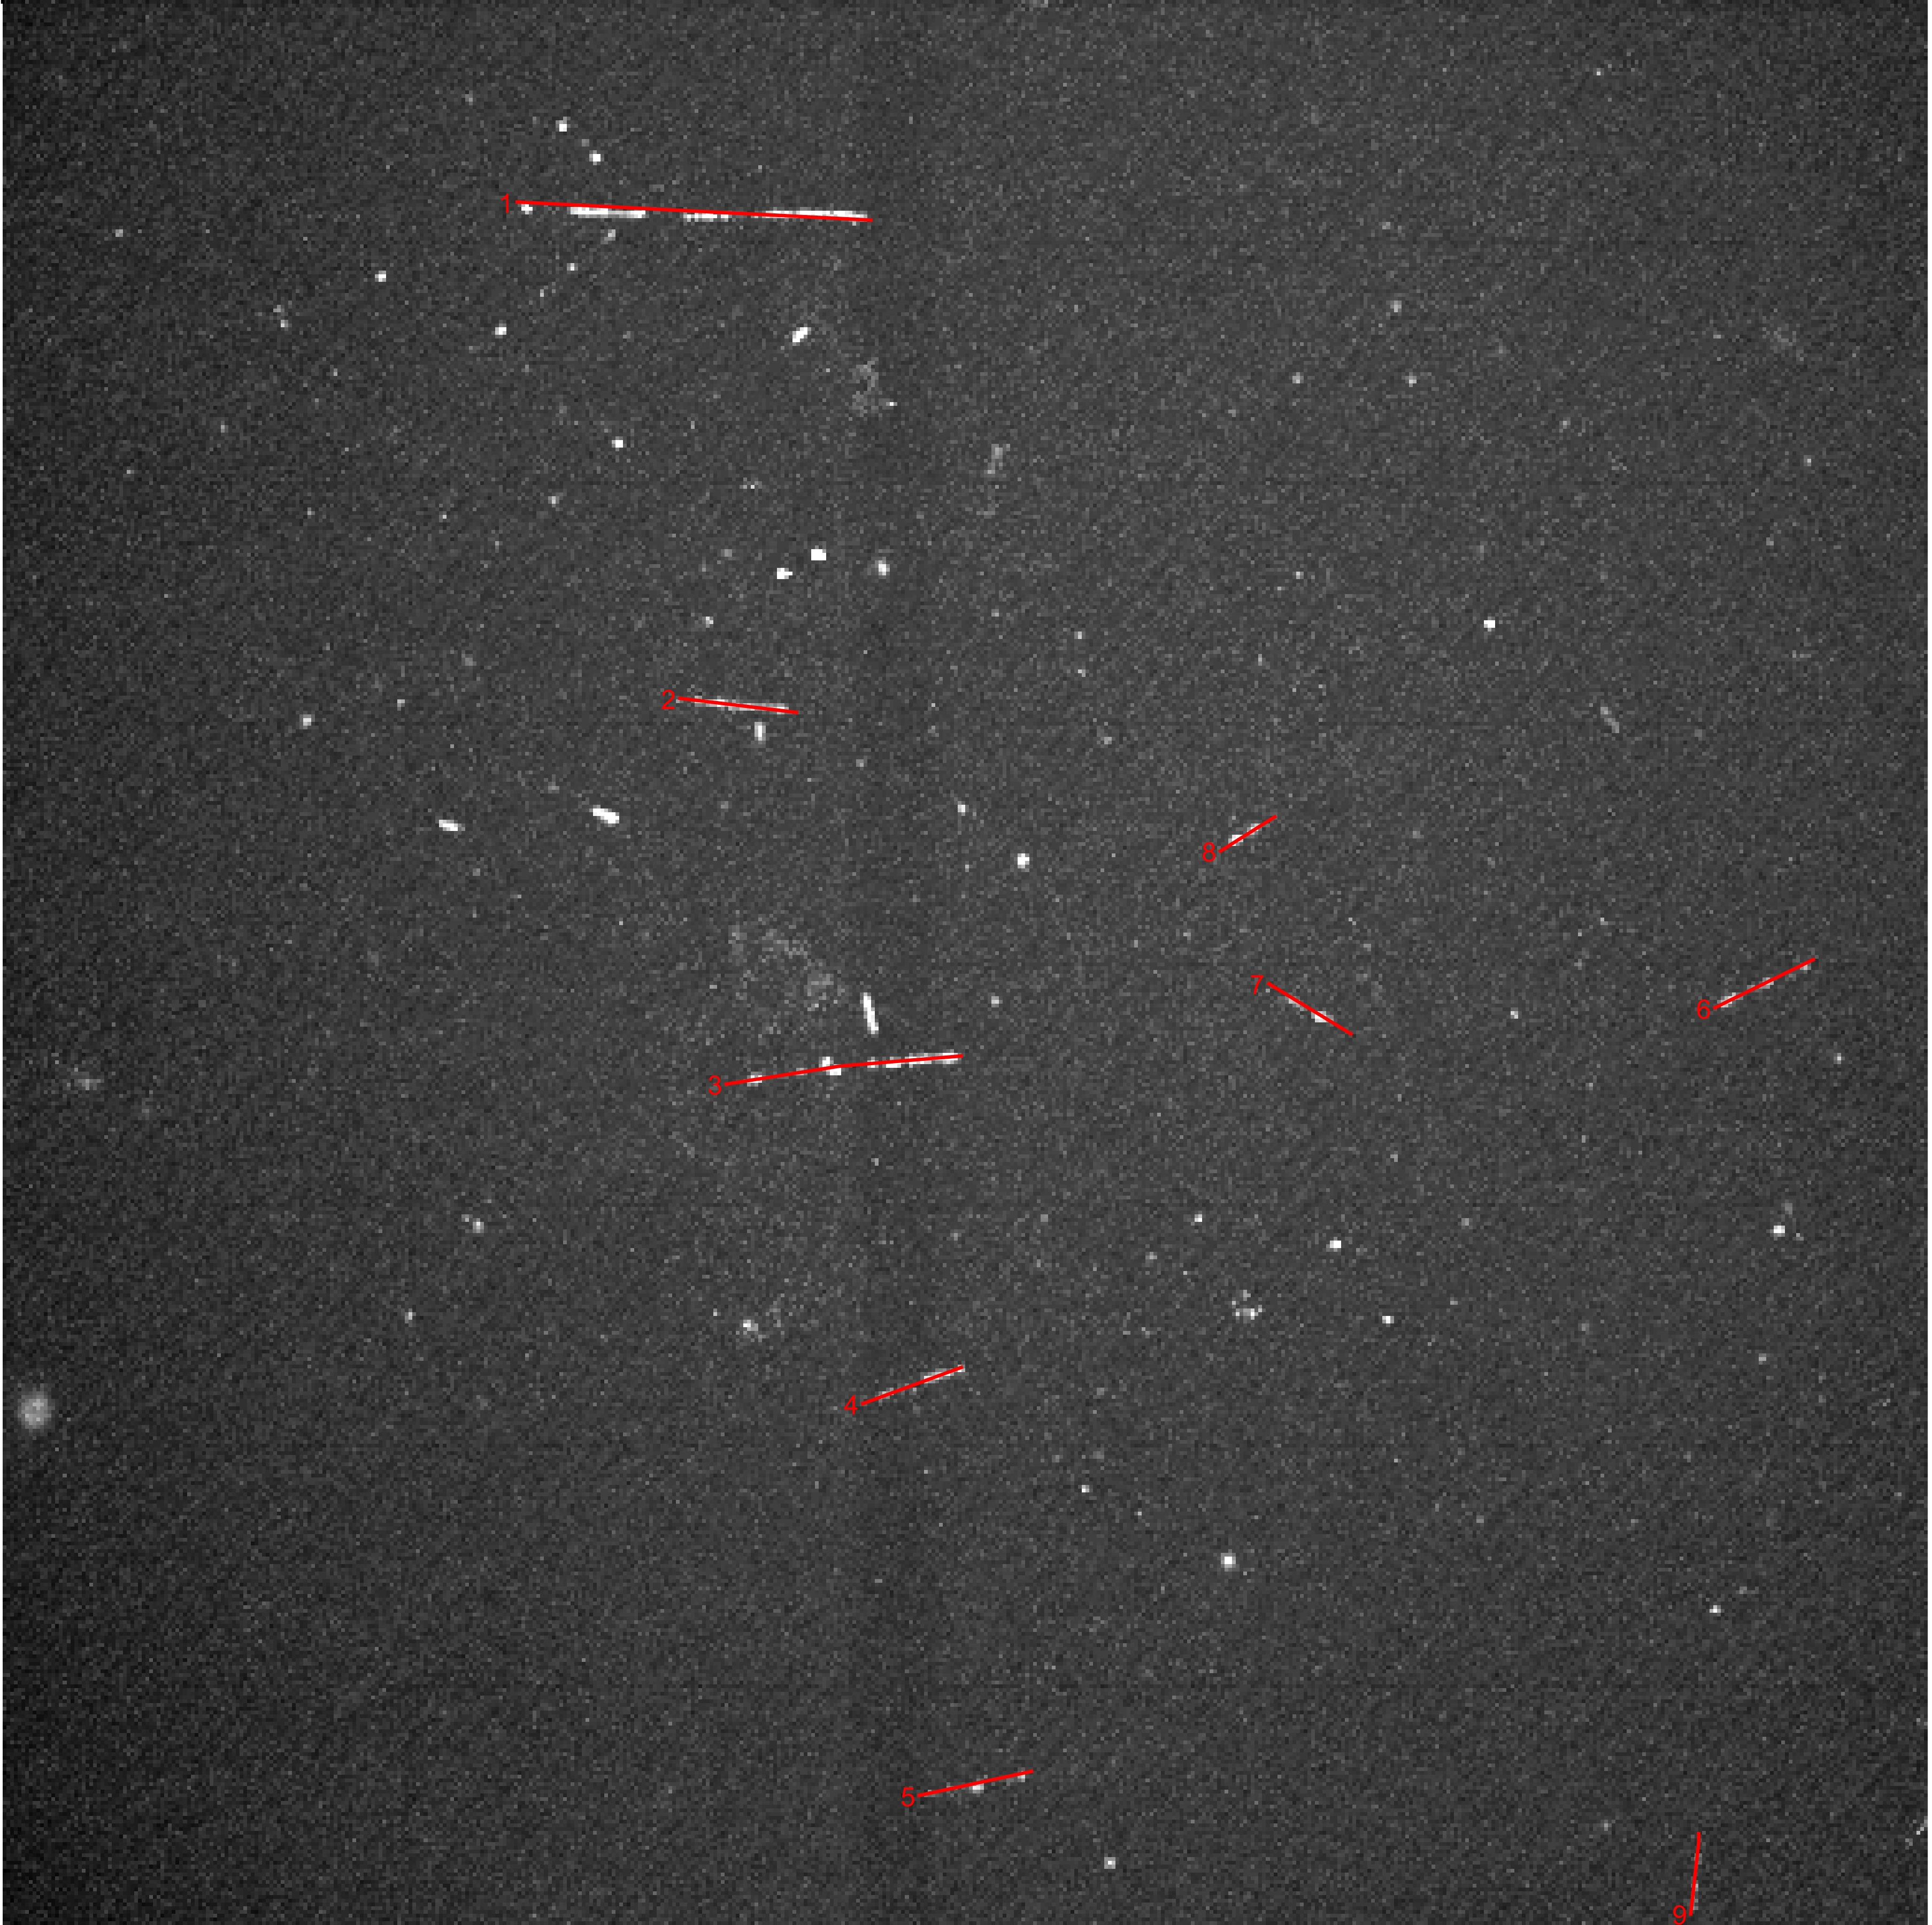
\includegraphics[scale=0.05]{pic/example_marked_tubules.jpg}
                        \captionof{figure}{first step marking of the microtubules}
                        \label{exp:markex1}
                   \minipend 
                   &
                   \minipanf
                     \begin{center}
                       \includegraphics[scale=0.0333]{pic/example_distances_time_marked.jpg}
                       \captionof{figure}{marking of the trajectories of the motor proteins}
                       \label{exp:markex2}
                     \end{center}
                   \minipend
                \end{tabular}    
        \end{center}
		% experimental procedure
\section{Data Analysis}
\subsection{Data evaluation of velocity}
\subsection{Data evaluation of run length}	% data analysis
\section{Discussion and conclusions}
%todo discuss 2.2 und 3.1/2 then add appendix 020325
	In this experiment we quantified the \textit{velocity} $v$ and the characteristic \textit{run length} $d$ (confidence level: $68.27\ \unit{\%}$) of \textit{Kinesin-1 motor proteins} by doing a kinesin-1 stepping assay:	
	\begin{align*}
	&v = (0.87 \pm 0.05)\ \unit{\mu m / s}\\
	&d = (1.1 \pm 0.2)\ \unit{\mu m}
	\end{align*} 
	Those results fit good to the values given in literature: $v_{lit} = 0.8\ \unit{\mu m/s}$\cite{PA} and $D_{lit} = 0.8\ \unit{\mu m}$\cite{runLength}.	% Auswertung bzw. Zusammenfassung
\input{MMC_protocol_appendix}    % Messprotokoll/Anhang
\section{References}

\begin{thebibliography}{99}
\bibitem [01] {PA} S. Diez. \textit{Advanced practical course - Experiment MMC}, Dresden, 2015
\bibitem [02] {wikiHisto} \texttt{https://en.wikipedia.org/wiki/Histogram} [November 20, 2015]
\bibitem [03] {wikiKinesin} \texttt{https://en.wikipedia.org/wiki/Kinesin} [November 22, 2015]
\bibitem [04] {runLength} S. Ferbrugge et al. \textit{Novel ways to determine kinesin-1's run length and randomness using fluorescence microscopy}. Amsterdam. October 2009
\bibitem [05] {severalMP} S. Klumpp, R. Lipowsky.\textit{Cooperative cargo transport by several molecular motors}. Potsdam. November 2005
\end{thebibliography}

\end{document}